\documentclass[11pt,a4paper]{article}
\usepackage{iftex}
\ifPDFTeX
  \usepackage[T1]{fontenc}
  \usepackage[utf8]{inputenc}
  \usepackage{lmodern}
  \renewcommand{\familydefault}{\sfdefault}
\else
  \usepackage{fontspec}
  \setmainfont{lmsans10-regular}[Extension=.otf,BoldFont=lmsans10-bold,ItalicFont=lmsans10-oblique,BoldItalicFont=lmsans10-boldoblique]
  \setmonofont{lmmono10-regular}[Extension=.otf]
\fi
\usepackage{babel}
\babelprovide[import,main]{french}
\usepackage[a4paper,margin=1.9cm,top=1.7cm,bottom=1.8cm]{geometry}
\usepackage{amsmath,amssymb,mathtools}
\usepackage{booktabs,array,tabularx}
\usepackage{microtype}
\usepackage[table]{xcolor}
\usepackage{tcolorbox}
\usepackage{enumitem}
\usepackage{fancyhdr,lastpage}
\usepackage{titlesec}
\usepackage{graphicx}
\usepackage{caption}
\captionsetup{font={small,color=Muted},labelfont={bf,color=Forest},skip=3pt}
\usepackage{hyperref}
\definecolor{Forest}{HTML}{174F43}
\definecolor{Sage}{HTML}{EDF2E6}
\definecolor{Ink}{HTML}{243C35}
\definecolor{Muted}{HTML}{65756A}
\definecolor{Amber}{HTML}{80633D}
\definecolor{Sand}{HTML}{FBF1E3}
\hypersetup{colorlinks=true,linkcolor=Forest,urlcolor=Forest,pdfauthor={Projet Clair},pdflang={fr-FR}}
\color{Ink}
\setlength{\parindent}{0pt}
\setlength{\parskip}{6pt}
\setlength{\headheight}{15pt}
\setlength{\emergencystretch}{2em}
\linespread{1.08}
\setlist[itemize]{leftmargin=1.3em,itemsep=3pt,topsep=4pt}
\setlist[enumerate]{leftmargin=1.5em,itemsep=4pt,topsep=4pt}
\titleformat{\section}{\Large\bfseries\color{Forest}}{\thesection}{.65em}{}
\titleformat{\subsection}{\normalsize\bfseries\color{Forest}}{}{0pt}{}
\titlespacing*{\section}{0pt}{9pt}{8pt}
\titlespacing*{\subsection}{0pt}{9pt}{3pt}
\newtcolorbox{keybox}{colback=Sage,colframe=Sage,boxrule=0pt,arc=3mm,left=3mm,right=3mm,top=2mm,bottom=2mm}
\newtcolorbox{limitbox}{colback=Sand,colframe=Sand,boxrule=0pt,arc=3mm,left=3mm,right=3mm,top=2mm,bottom=2mm}
\newcommand{\E}{\mathbb E}
\newcommand{\Var}{\operatorname{Var}}
\newcommand{\Cov}{\operatorname{Cov}}
\newcommand{\G}{\operatorname{Gamma}}
\newcommand{\Pois}{\operatorname{Poisson}}
\newcommand{\NB}{\operatorname{NB2}}
\newcommand{\RMSEP}{\operatorname{RMSEP}}
\newcommand{\MSEP}{\operatorname{MSEP}}
\newcommand{\smallnote}[1]{{\small\color{Muted}#1}}
\pagestyle{fancy}
\fancyhf{}
\fancyhead[L]{\small\bfseries\color{Forest}CLAIR / NOTE MÉTHODOLOGIQUE}
\fancyhead[R]{\small\color{Muted}Version du 12 novembre 2026}
\fancyfoot[L]{\footnotesize\color{Muted}Méthodes implémentées, résultats mesurés, limites explicites.}
\fancyfoot[R]{\footnotesize\color{Forest}\thepage\,/\,\pageref{LastPage}}
\renewcommand{\headrulewidth}{0pt}
\renewcommand{\footrulewidth}{0pt}
\hypersetup{pdftitle={Clair — Tarification automobile : modèles et validation}}
\begin{document}
{\small\color{Muted}\textbf{NOTE 01}\quad TARIFICATION AUTOMOBILE}
\vspace{5mm}

{\fontsize{27}{31}\selectfont\bfseries\color{Forest}Du profil assuré\par à une prime expliquée.}

{\large GLM, Poisson et binomiale négative, prime bayésienne\par et crédibilité sur les coûts.}
\vspace{3mm}

\begin{keybox}
\textbf{Objectif.} Estimer le coût attendu des sinistres d'un contrat, puis ajuster cette estimation à son expérience. Le projet comprend un moteur Python, son équivalent navigateur et une interface métier.
\end{keybox}

\section*{Ce qui est effectivement réalisé}
\begin{itemize}
\item Audit de la source originale \texttt{freMTPL2} : \textbf{677\,991 contrats} et \textbf{26\,444 sinistres}, sans incohérence entre les nombres et les montants disponibles.
\item GLM Poisson pour la fréquence et Gamma pour le coût moyen ; comparaison d'un challenger NB2 et d'une sévérité plafonnée avec recharge des excédents.
\item Calibration de l'hétérogénéité Poisson--Gamma ; prime bayésienne et crédibilité \emph{structurelle} calculables depuis un historique saisi.
\item Coefficients versionnés, exports traçables, tests de calcul et de parité Python/navigateur.
\end{itemize}

\subsection*{Un protocole séparant estimation et évaluation}
\begin{center}
\begin{tabular}{lrrr}
\toprule
& Apprentissage & Validation & Test \\
\midrule
Contrats & 407\,317 & 135\,471 & 135\,203 \\
Sinistres & 15\,909 & 5\,302 & 5\,233 \\
\bottomrule
\end{tabular}
\end{center}
Découpage stable par identifiant de contrat : environ 60\,/\,20\,/\,20. Les sinistres suivent le découpage de leur contrat. La préparation est ajustée sur l'apprentissage ; les variantes sont choisies sur la validation. Le test initial ne sert pas au réglage.

\begin{limitbox}
\textbf{Résultat de validation à conserver.} Sur le test : \textbf{10,33 M\texteuro{} observés contre 12,54 M\texteuro{} prédits}. Le ratio de charge observée/prédite est de \textbf{82,4\,\%}. Le projet est un démonstrateur calibré sur données historiques, sans approbation de tarif commercial actuel.
\end{limitbox}

\smallnote{Source : CASdatasets, commit \texttt{227fb56b8734bdb7c0327a41180e01d2ddaeaf26}. Données approximativement 2011--2013. Modèle : \texttt{fremtpl2-2026-11-v1}. Les montants ne sont pas automatiquement actualisés aux conditions économiques de 2026.}

\newpage
\section{Construire la prime pure avec deux GLM}
Pour un assuré $i$, $x_i$ décrit le profil, $e_i$ l'exposition en années, $N_i$ le nombre de sinistres et $Y_{ik}$ leur coût. La charge est
\[
S_i=\sum_{k=1}^{N_i}Y_{ik}.
\]
Sous indépendance conditionnelle du nombre et des coûts, avec des coûts de même espérance,
\[
\boxed{\E[S_i\mid x_i,e_i]=e_i\lambda_i m_i,\qquad \pi_i^0=\lambda_i m_i.}
\]
$\pi_i^0$ est la prime pure \emph{annuelle}. $e_i\pi_i^0$ est la charge attendue sur la période.

\subsection*{Famille exponentielle et lien logarithmique}
\[
f(y;\theta,\phi)=\exp\!\left\{\frac{y\theta-b(\theta)}{a(\phi)}+c(y,\phi)\right\},
\quad \E[Y]=b'(\theta),\quad \Var(Y)=a(\phi)b''(\theta).
\]
Un GLM pose $g(\mu_i)=x_i^\top\beta$. Avec $g=\log$, la moyenne vaut $\exp(x_i^\top\beta)>0$. Cela ne suppose pas une \emph{loi exponentielle} pour les observations.

\subsection*{Fréquence : Poisson avec exposition}
\[
N_i\mid x_i,e_i\sim\Pois(\mu_i),\quad
\lambda_i=\exp(x_i^\top\beta_N),\quad
\log\mu_i=\underbrace{\log e_i}_{\text{offset}}+x_i^\top\beta_N.
\]
L'ajustement sur $N_i/e_i$, pondéré par $e_i$, donne les mêmes équations de moyenne. Le coefficient de l'offset est fixé à 1 ; l'exposition n'est pas une variable explicative libre.

\subsection*{Sévérité : Gamma à lien log}
Pour chaque sinistre strictement positif :
\[
Y_{ik}\mid x_i\sim\G\!\left(\text{forme}=\frac1{\phi_Y},\ \text{taux}=\frac1{\phi_Ym_i}\right),
\quad m_i=\exp(x_i^\top\beta_Y),\quad \Var(Y_{ik}\mid x_i)=\phi_Ym_i^2.
\]
La convention est \emph{forme/taux}. Le lien log de la Gamma est valide et non canonique. Les coefficients de moyenne sont ajustés par minimisation de la perte Gamma, éventuellement pénalisée en $L^2$. Un facteur de niveau est calculé sur l'apprentissage uniquement pour équilibrer la somme des coûts prédits par sinistre.

\smallnote{Variables : tranches d'âge conducteur et véhicule, puissance fiscale, carburant, zone et région historique. L'identifiant est exclu. Le bonus-malus est exclu pour éviter de réutiliser explicitement le même historique dans l'ajustement a posteriori. Les bornes sont fixes ; l'encodage est ajusté sur l'apprentissage.}

\section{Poisson, NB2 et validation de la charge}
\begin{figure}[htbp]
\centering
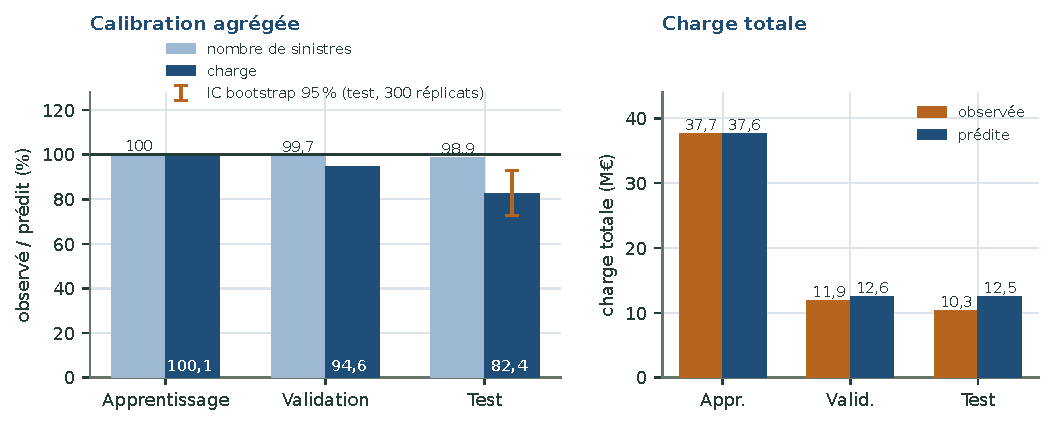
\includegraphics[width=\linewidth]{figures/fig_calibration.pdf}
\caption{Calibration agrégée par échantillon. Le nombre de sinistres est bien reproduit (98,9\,\% sur le test), mais la charge prédite dépasse la charge observée sur le test : le ratio observé/prédit tombe à 82,4\,\%, avec un intervalle bootstrap de 72,6 à 92,8\,\%. Le défaut vient de la sévérité, pas de la fréquence.}\label{fig:calibration}
\end{figure}

\subsection*{Une variance plus souple ne garantit pas une meilleure prime}
Pour une même forme de moyenne $\mu_i=e_i\exp(x_i^\top\beta)$ :
\[
\begin{aligned}
\text{Poisson :}\qquad &\Var(N_i\mid x_i,e_i)=\mu_i,\\
\text{NB2 :}\qquad &\Var(N_i\mid x_i,e_i)=\mu_i+\mu_i^2/r,\quad r>0.
\end{aligned}
\]
La dispersion de Pearson du Poisson sur apprentissage vaut environ $1{,}764$. Le challenger NB2 réestime conjointement $\beta$ et $r$ par maximum de vraisemblance, en conservant le modèle de coût. Il donne $\widehat r\simeq0{,}6950$.

\begin{center}
\small
\begin{tabularx}{\linewidth}{Xrr}
\toprule
Indicateur & Poisson & NB2 \\
\midrule
Log-vraisemblance négative moyenne, validation & 0,162524 & 0,161743 \\
O/P nombre, test déjà consulté & 98,92\,\% & 98,07\,\% \\
O/P charge, test déjà consulté & 82,41\,\% & 81,56\,\% \\
Déviance Tweedie de prime pure, test & 80,511 & 80,544 \\
\bottomrule
\end{tabularx}
\end{center}
\textbf{Décision mesurée :} conserver Poisson comme référence. La NB2 améliore ici la description probabiliste des nombres, mais pas la prime pure. Le test ayant déjà été vu, cette comparaison supplémentaire est un diagnostic, pas une nouvelle validation indépendante.

\begin{figure}[htbp]
\centering
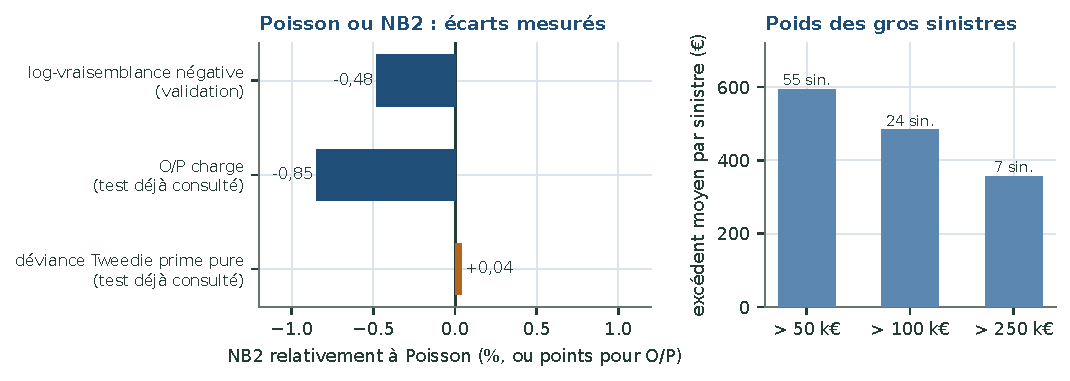
\includegraphics[width=\linewidth]{figures/fig_diagnostics.pdf}
\caption{À gauche, écarts mesurés entre la binomiale négative et le Poisson : ils sont d'ordre inférieur au pourcent et ne justifient pas un changement de modèle. À droite, excédent moyen par sinistre au-delà de chaque seuil sur l'apprentissage : quelques dizaines de sinistres pèsent sur la moyenne de toute la base.}\label{fig:diagnostics}
\end{figure}

\subsection*{Le point sensible : les gros sinistres}
Le coût moyen observé est d'environ \textbf{2\,367\texteuro{}} en apprentissage, \textbf{2\,248\texteuro{}} en validation et \textbf{1\,974\texteuro{}} en test. Les dix plus gros sinistres représentent \textbf{21,4\,\%} de la charge d'apprentissage.

La dispersion Gamma estimée par vraisemblance est $\widehat\phi_Y\simeq1{,}3154$, alors que le second moment relatif empirique atteint environ $30{,}0965$. Cet écart signale que la Gamma ajustée ne décrit pas bien toute la queue des coûts.

Une variante a testé un plafond à 100\,000\texteuro{} avec recharge des excédents. Elle n'a pas été retenue sur la validation. La décomposition à étudier reste
\[
\E[Y\mid x]=\E[\min(Y,u)\mid x]+\E[(Y-u)_+\mid x].
\]
\begin{limitbox}
Un plafonnement sans recharge change la cible. Multiplier les primes par le ratio 0,824 observé sur le test ferait aussi perdre l'indépendance de cette évaluation. Les corrections futures doivent être choisies ailleurs, puis évaluées sur de nouvelles données.
\end{limitbox}

\begin{figure}[htbp]
\centering
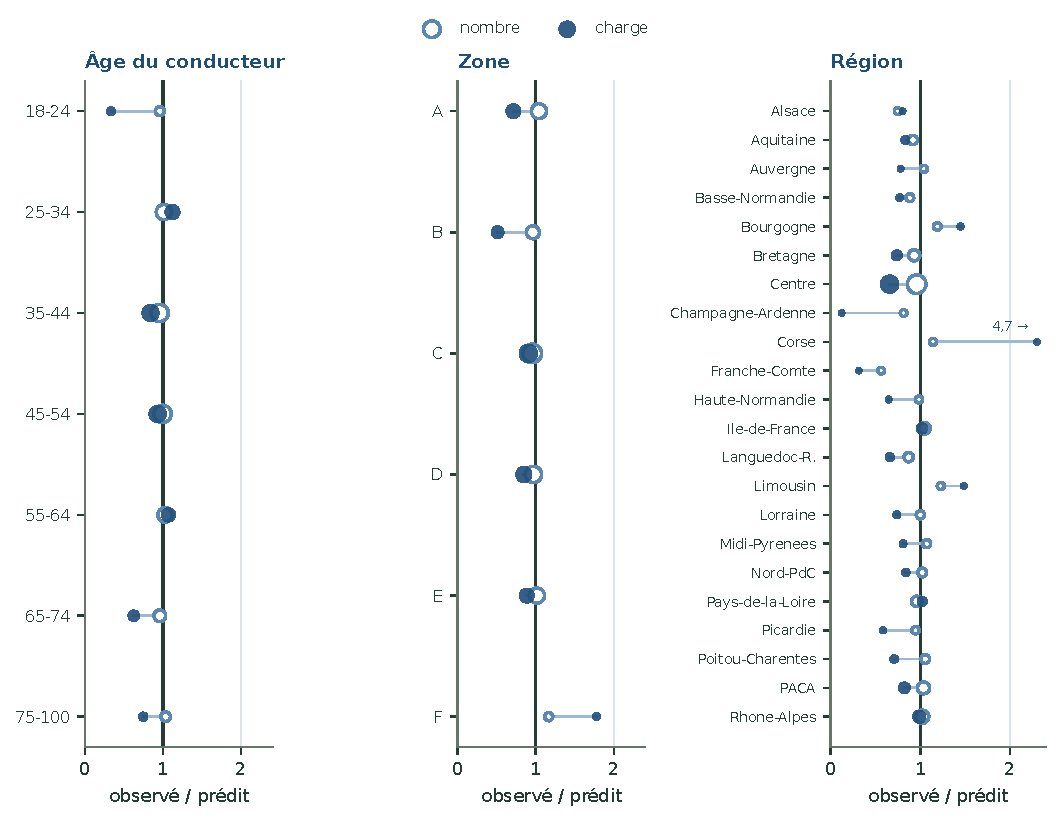
\includegraphics[width=\linewidth]{figures/fig_segments.pdf}
\caption{Rapport observé/prédit par segment du jeu de test. Un point creux est le nombre de sinistres, un point plein la charge ; la surface est proportionnelle à l'exposition. Le ratio du nombre reste à $\pm10\,\%$ de 1 pour 26 segments sur 35, celui de la charge pour 6 seulement ; l'écart est le plus fort dans les segments à faible exposition (Corse : 4,7, valeur tronquée sur la figure).}\label{fig:segments}
\end{figure}

\section{Prime bayésienne : apprendre du nombre}
\subsection*{Un effet individuel multiplicatif}
La fréquence du GLM décrit la moyenne du profil. On introduit un risque latent $U_i$ :
\[
U_i\mid x_i\sim\G(r,r),\qquad \E[U_i]=1,\quad\Var(U_i)=1/r,
\]
\[
N_i(t_i)\mid U_i,x_i\sim\Pois(t_i\lambda_iU_i).
\]
En intégrant $U_i$, le nombre suit une NB2. La surdispersion est donc cohérente avec une hétérogénéité individuelle, sans prouver que celle-ci persiste dans le temps.

Le modèle livré estime $r$ par vraisemblance marginale sur l'apprentissage, \emph{en maintenant les moyennes du GLM Poisson figées} : $\widehat r\simeq0{,}6984$. Cette estimation diffère du $r$ du challenger NB2, où les coefficients sont réestimés conjointement.

\subsection*{Conjugaison et fréquence ajustée}
Après observation de $n_i$ sinistres sur $t_i$ années assurées, à profil comparable :
\[
\boxed{U_i\mid n_i,t_i,x_i\sim\G(r+n_i,\ r+t_i\lambda_i).}
\]
La fréquence annuelle future ajustée est
\[
\widetilde\lambda_i=\lambda_i\frac{r+n_i}{r+t_i\lambda_i}
=\frac{\alpha_i+n_i}{\beta_i+t_i},
\quad \alpha_i=r,\quad\beta_i=\frac r{\lambda_i}.
\]
Le coût moyen $m_i$ reste celui du modèle initial :
\[
\boxed{\pi_i^B=m_i\frac{\alpha_i+n_i}{\beta_i+t_i}
=(1-Z_i)\pi_i^0+Z_i\,m_i\frac{n_i}{t_i},\qquad
Z_i=\frac{t_i}{\beta_i+t_i}.}
\]
L'écriture de droite vaut pour $t_i>0$. Sans historique, la formule de gauche redonne $\pi_i^0$.

\begin{keybox}
\textbf{Illustration calculée, historique fictif.} Profil : conducteur de 45 ans, véhicule de 7 ans, 6 CV, diesel, zone C, région Centre. Le modèle donne $\lambda\simeq0{,}08054$, $m\simeq1\,959{,}86$ et $\beta\simeq8{,}672$.

Prime pure initiale : \textbf{157,84\texteuro{}/an}. En supposant trois années sans sinistre, la prime bayésienne vaut \textbf{117,27\texteuro{}/an}, dans la base économique historique du modèle.
\end{keybox}
\begin{figure}[htbp]
\centering
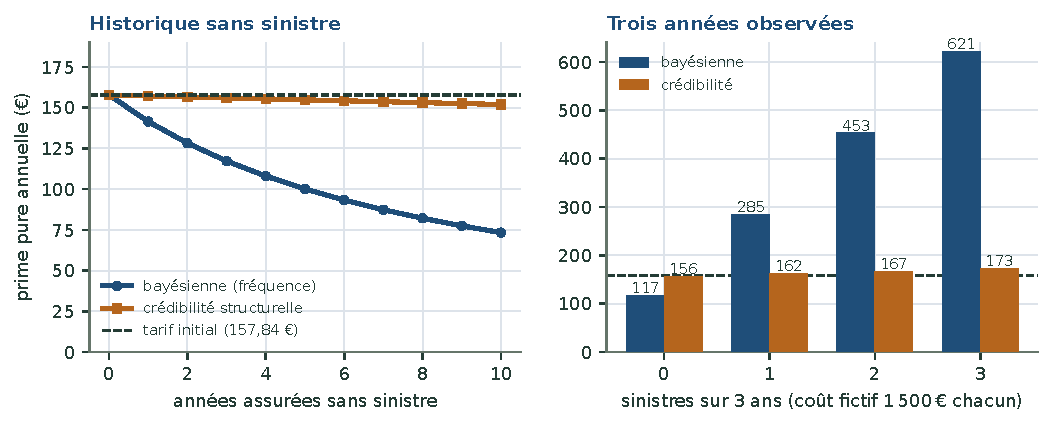
\includegraphics[width=\linewidth]{figures/fig_personalisation.pdf}
\caption{Personnalisation pour le profil illustré (conducteur de 45 ans). À gauche, la prime bayésienne baisse vite avec les années sans sinistre ; la crédibilité structurelle, avec $K\simeq261$ années, bouge à peine. À droite, effet de sinistres fictifs sur trois ans. Les historiques sont des exemples de calcul, pas des données observées.}\label{fig:personalisation}
\end{figure}

\smallnote{Cette version ajuste la fréquence, pas la sévérité individuelle. Elle suppose un profil comparable sur l'historique et la période future. La performance de renouvellement n'est pas validée sur un panel longitudinal.}

\section{Crédibilité : apprendre des coûts}
\subsection*{Le cadre non paramétrique de référence}
Pour une charge annuelle $X$ et un risque latent $\Theta$, on définit
\[
v=\E[\Var(X\mid\Theta)],\qquad
 a=\Var(\E[X\mid\Theta]),\qquad K=v/a.
\]
La prime de crédibilité de Bühlmann s'écrit
\[
\pi^C=(1-Z)\mu+Z\overline X,\qquad Z=\frac t{t+K}.
\]
Estimer $v$ et $a$ non paramétriquement exige des observations répétées de risques comparables. La seule coupe annuelle \texttt{freMTPL2} ne fournit pas cette validation longitudinale.

\subsection*{Ce qui est implémenté : une crédibilité structurelle}
Sous le modèle collectif avec fréquence $\lambda_iU_i$, coûts conditionnellement indépendants et moyenne $m_i$ :
\[
v_i=\lambda_i\E[Y^2\mid x_i],\qquad
 a_i=\lambda_i^2m_i^2/r.
\]
On en déduit
\[
\boxed{K_i=\frac r{\lambda_i}\,q_i,\qquad
q_i=\frac{\E[Y^2\mid x_i]}{m_i^2}.}
\]
Le moteur estime sur l'apprentissage un second moment relatif commun aux profils :
\[
\widehat q=\frac1{M_{\rm train}}\sum_{k\in\mathrm{train}}
\left(\frac{Y_k}{\widehat m(x_k)}\right)^2\simeq30{,}0965.
\]
Il suppose donc une stabilité du second moment relatif entre profils, à vérifier. Cette estimation empirique de queue n'est pas remplacée par le moment théorique $1+\widehat\phi_Y$ de la Gamma ajustée.

Pour une charge historique totale $S_i^{\rm hist}$ et une exposition totale $t_i$ :
\[
\boxed{\pi_i^C=(1-Z_i)\pi_i^0+Z_i\frac{S_i^{\rm hist}}{t_i},\qquad
 Z_i=\frac{t_i}{t_i+K_i}.}
\]
Pour des périodes partielles, cette pondération suppose une variance du coût annualisé inversement proportionnelle à l'exposition, comme dans une extension de type Bühlmann--Straub.

\begin{keybox}
Sur le profil illustré précédemment, $K\simeq260{,}996$ années. Avec trois années sans sinistre, la prime de crédibilité vaut \textbf{156,05\texteuro{}/an}. Le faible poids des coûts individuels reflète ici leur forte variabilité et les hypothèses structurelles ; il ne s'agit pas d'un réglage arbitraire $K=4$.
\end{keybox}

\section{Du coût attendu au montant proposé}
\subsection*{Base économique et durée de couverture}
Le tarif est exprimé dans la base économique historique de la source. Si le métier fournit un facteur d'évolution des coûts $I$, le moteur utilise $m_i^{\rm cible}=I\,m_i$. Ce facteur doit être justifié ; $I=1$ n'actualise rien. Les charges historiques saisies doivent être exprimées dans la même base.

Pour une exposition future $e_i^\star$ et la prime annuelle retenue $\pi_i$ :
\[
P_i^{\rm pure}=e_i^\star\pi_i.
\]
Avec des frais fixes $F$, un taux de frais variables $f$ et une marge $g$, exprimés en proportions du montant HT :
\[
P_i^{HT}=P_i^{\rm pure}+F+(f+g)P_i^{HT},\qquad
\boxed{P_i^{HT}=\frac{e_i^\star\pi_i+F}{1-f-g}},\quad f+g<1.
\]
Ces chargements sont des hypothèses métier, initialisées à zéro. La base de sinistres ne permet pas de calibrer les frais compagnie, la fiscalité, la réassurance ou les objectifs de capital. La mensualisation affichée est un quotient, sans frais de fractionnement.

\subsection*{Traçabilité et contrôles livrés}
\begin{itemize}
\item Source figée, empreintes des fichiers, versions des dépendances et coefficients exportés.
\item Contrôles de domaine : âges, puissance, modalités, expositions et nombres entiers.
\item Séparation annuel/période ; historique sans exposition refusé ; absence d'historique correctement traitée.
\item Parité Python/navigateur vérifiée sur 36 situations de calcul et 24 profils synthétiques.
\item Dossier JSON contenant version du modèle, empreinte, hypothèses, profil et résultats ; absence de stockage automatique des historiques dans l'application.
\end{itemize}

\begin{limitbox}
\textbf{Avant un usage compagnie :} obtenir un portefeuille récent avec garanties et maturité des coûts comparables ; revoir la queue de sévérité ; acquérir un panel de renouvellements ; fixer les hypothèses économiques ; obtenir une revue actuarielle indépendante. Le test actuel est connu et ne peut plus servir d'évaluation finale indépendante d'un nouveau réglage.
\end{limitbox}

\subsection*{Code, résultats et références}
\small
\begin{itemize}[itemsep=2pt]
\item \href{https://github.com/kelian19/assurance-tarification}{Dépôt : kelian19/assurance-tarification}. Voir \texttt{reports/MODEL\_CARD.md}, \texttt{reports/POISSON\_VS\_NB.md} et \texttt{artifacts/model.json}.
\item \href{https://dutangc.github.io/CASdatasets/reference/freMTPL.html}{CASdatasets : documentation freMTPL2}.
\item \href{https://scikit-learn.org/stable/auto_examples/linear_model/plot_tweedie_regression_insurance_claims.html}{Scikit-learn : fréquence, sévérité et régression Tweedie}.
\item \href{https://www.statsmodels.org/stable/generated/statsmodels.discrete.discrete_model.NegativeBinomial.html}{Statsmodels : paramétrisation NB2}.
\item Nicolas Baradel, \emph{Mathématiques de l'assurance dommages}, cours fourni, version du 8 septembre 2026, p. 3--24.
\end{itemize}
\end{document}
